\apendice{Especificación de requisitos}
\section{Diagrama de casos de uso}
Los diagramas de casos de uso ayudan en la comprensión general de las posibles interacciones entre los pacientes y las funciones ofrecidas por la web, como se muestra en la Figura \ref{fig:diagrama}.

\begin{figure}[h]
\centering
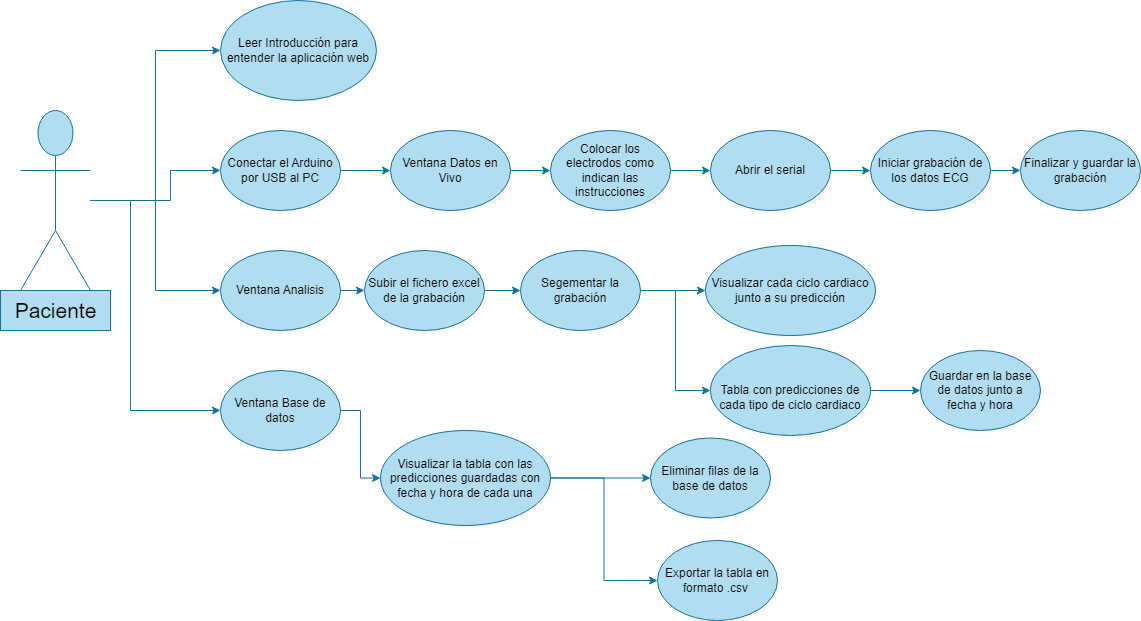
\includegraphics[width=1\textwidth]{img/Diagramas/casosdeuso.drawio (1).png}
\caption{Funciones para todos los usuarios}
\label{fig:diagrama}
\end{figure}

\section{Explicación casos de uso}


La sección de casos de uso describe cómo los usuarios interactúan con la aplicación y qué esperar de ella. Esta parte ayuda a entender qué hace cada parte del sistema, como si fuera una guía paso a paso de cada función. Al explicar las acciones en términos simples, cualquier persona, sin importar su conocimiento técnico, puede comprender cómo usar la aplicación y qué funciones están disponibles. Es como leer un manual de instrucciones que nos muestra cómo aprovechar al máximo el sistema.




% Caso de Uso 1 -> Introducción.
\begin{table}[p]
	\centering
	\begin{tabularx}{\linewidth}{ p{0.21\columnwidth} p{0.71\columnwidth} }
		\toprule
		\textbf{CU-1}    & \textbf{Introducción}\\
		\toprule
		\textbf{Versión}              & 2.0    \\
		\textbf{Autor}                & Diego Trascasa García \\
		\textbf{Requisitos asociados} & RF-01 \\
		\textbf{Descripción}          & Presenta una explicación del funcionamiento de la web y sus funcionalidades. \\
		\textbf{Precondición}         & Ninguna. \\
		\textbf{Acciones}             &
		\begin{enumerate}
			\item El usuario accede a la página web.
			\item Visualiza la sección de introducción donde se explican las funcionalidades de la web.
		\end{enumerate}\\
		\textbf{Postcondiciones}      & 
		\begin{enumerate}
			\item El usuario entiende cómo utilizar la web.
		\end{enumerate}\\
		\textbf{Excepciones}          & 
		\begin{enumerate}
			\item Ninguna.
		\end{enumerate}\\
		\textbf{Importancia}          & Alta \\
		\bottomrule
	\end{tabularx}
	\caption{CU-1 Introducción.}
    \label{CU-1}
\end{table}

% Caso de Uso 2 -> Instrucciones para encender el prototipo y colocar los electrodos.
\begin{table}[p]
	\centering
	\begin{tabularx}{\linewidth}{ p{0.21\columnwidth} p{0.71\columnwidth} }
		\toprule
		\textbf{CU-2}    & \textbf{Instrucciones para encender el prototipo y colocar los electrodos}\\
		\toprule
		\textbf{Versión}              & 2.0    \\
		\textbf{Autor}                & Diego Trascasa García \\
		\textbf{Requisitos asociados} & RF-02, RF-03 \\
		\textbf{Descripción}          & Proporciona instrucciones para usar el prototipo y visualizar los datos de ECG en tiempo real. \\
		\textbf{Precondición}         & Prototipo encendido y electrodos correctamente colocados. \\
		\textbf{Acciones}             &
		\begin{enumerate}
			\item El usuario sigue las instrucciones para encender el prototipo.
			\item Coloca los electrodos según las indicaciones.
			\item Abre la ventana de escritorio de Tkinter para visualizar los datos de ECG en tiempo real.
			\item Graba los datos si es necesario.
		\end{enumerate}\\
		\textbf{Postcondiciones}      & 
		\begin{enumerate}
			\item Datos de ECG visualizados en tiempo real.
		\end{enumerate}\\
		\textbf{Excepciones}          & 
		\begin{enumerate}
			\item Prototipo no enciende.
			\item Electrodos mal colocados.
			\item Problemas con la visualización en Tkinter.
		\end{enumerate}\\
		\textbf{Importancia}          & Alta \\
		\bottomrule
	\end{tabularx}
	\caption{CU-2 Instrucciones para encender el prototipo y colocar los electrodos.}
    \label{CU-2}
\end{table}

% Caso de Uso 3 -> Abrir/Cerrar Serial.
\begin{table}[p]
	\centering
	\begin{tabularx}{\linewidth}{ p{0.21\columnwidth} p{0.71\columnwidth} }
		\toprule
		\textbf{CU-3}    & \textbf{Abrir/Cerrar Serial}\\
		\toprule
		\textbf{Versión}              & 2.0    \\
		\textbf{Autor}                & Diego Trascasa García \\
		\textbf{Requisitos asociados} & RF-03 \\
		\textbf{Descripción}          & Permite abrir y cerrar la comunicación serial con el prototipo. \\
		\textbf{Precondición}         & Prototipo conectado al puerto USB. \\
		\textbf{Acciones}             &
		\begin{enumerate}
			\item El usuario conecta el prototipo al puerto USB.
			\item Abre la aplicación web.
			\item Selecciona la opción para abrir la comunicación serial.
			\item Realiza las operaciones necesarias.
			\item Selecciona la opción para cerrar la comunicación serial.
		\end{enumerate}\\
		\textbf{Postcondiciones}      & 
		\begin{enumerate}
			\item Comunicación serial abierta o cerrada según la acción realizada.
		\end{enumerate}\\
		\textbf{Excepciones}          & 
		\begin{enumerate}
			\item Fallo en la conexión del prototipo al puerto USB.
			\item Error al intentar abrir o cerrar la comunicación serial.
		\end{enumerate}\\
		\textbf{Importancia}          & Alta \\
		\bottomrule
	\end{tabularx}
	\caption{CU-3 Abrir/Cerrar Serial.}
    \label{CU-3}
\end{table}

% Caso de Uso 4 -> Iniciar grabación de datos.
\begin{table}[p]
	\centering
	\begin{tabularx}{\linewidth}{ p{0.21\columnwidth} p{0.71\columnwidth} }
		\toprule
		\textbf{CU-4}    & \textbf{Iniciar grabación de datos}\\
		\toprule
		\textbf{Versión}              & 2.0    \\
		\textbf{Autor}                & Diego Trascasa García \\
		\textbf{Requisitos asociados} & RF-04 \\
		\textbf{Descripción}          & Permite al usuario iniciar la grabación de los datos de ECG desde el prototipo. \\
		\textbf{Precondición}         & Prototipo conectado y comunicación serial abierta. \\
		\textbf{Acciones}             &
		\begin{enumerate}
			\item El usuario abre la aplicación web.
			\item Selecciona la opción para iniciar la grabación de datos.
			\item El sistema comienza a registrar los datos de ECG recibidos del prototipo.
		\end{enumerate}\\
		\textbf{Postcondiciones}      & 
		\begin{enumerate}
			\item Los datos de ECG se están grabando y almacenando para su posterior análisis.
		\end{enumerate}\\
		\textbf{Excepciones}          & 
		\begin{enumerate}
			\item Fallo en la comunicación serial impide la grabación de datos.
			\item Error al intentar iniciar la grabación de datos.
		\end{enumerate}\\
		\textbf{Importancia}          & Alta \\
		\bottomrule
	\end{tabularx}
	\caption{CU-4 Iniciar grabación de datos.}
    \label{CU-4}
\end{table}


% Caso de Uso 5 -> Finalizar grabación de datos.
\begin{table}[p]
	\centering
	\begin{tabularx}{\linewidth}{ p{0.21\columnwidth} p{0.71\columnwidth} }
		\toprule
		\textbf{CU-5}    & \textbf{Finalizar grabación de datos}\\
		\toprule
		\textbf{Versión}              & 2.0    \\
		\textbf{Autor}                & Diego Trascasa García \\
		\textbf{Requisitos asociados} & RF-04 \\
		\textbf{Descripción}          & Permite al usuario detener la grabación de los datos de ECG desde el prototipo. \\
		\textbf{Precondición}         & Grabación de datos de ECG en curso. \\
		\textbf{Acciones}             &
		\begin{enumerate}
			\item El usuario abre la aplicación web.
			\item Selecciona la opción para finalizar la grabación de datos.
			\item El sistema detiene el registro de los datos de ECG.
		\end{enumerate}\\
		\textbf{Postcondiciones}      & 
		\begin{enumerate}
			\item Los datos de ECG grabados se almacenan para su posterior análisis.
		\end{enumerate}\\
		\textbf{Excepciones}          & 
		\begin{enumerate}
			\item Fallo en la comunicación serial impide la finalización correcta de la grabación de datos.
			\item Error al intentar detener la grabación de datos.
		\end{enumerate}\\
		\textbf{Importancia}          & Alta \\
		\bottomrule
	\end{tabularx}
	\caption{CU-5 Finalizar grabación de datos.}
    \label{CU-5}
\end{table}

% Caso de Uso 6 -> Subir archivo Excel para análisis.
\begin{table}[p]
	\centering
	\begin{tabularx}{\linewidth}{ p{0.21\columnwidth} p{0.71\columnwidth} }
		\toprule
		\textbf{CU-6}    & \textbf{Subir archivo Excel para análisis}\\
		\toprule
		\textbf{Versión}              & 2.0    \\
		\textbf{Autor}                & Diego Trascasa García \\
		\textbf{Requisitos asociados} & RF-05 \\
		\textbf{Descripción}          & Permite al usuario cargar un archivo Excel con datos de ECG para su análisis. \\
		\textbf{Precondición}         & Archivo Excel con datos de ECG disponible para cargar. \\
		\textbf{Acciones}             &
		\begin{enumerate}
			\item El usuario abre la aplicación web.
			\item Selecciona la opción para subir un archivo Excel.
			\item El usuario carga el archivo Excel desde su dispositivo.
			\item El sistema valida el formato del archivo y procesa los datos.
		\end{enumerate}\\
		\textbf{Postcondiciones}      & 
		\begin{enumerate}
			\item El archivo Excel es cargado exitosamente y los datos están listos para su análisis.
		\end{enumerate}\\
		\textbf{Excepciones}          & 
		\begin{enumerate}
			\item El archivo no es del formato esperado (no es Excel).
			\item El archivo Excel no contiene datos de ECG válidos.
		\end{enumerate}\\
		\textbf{Importancia}          & Alta \\
		\bottomrule
	\end{tabularx}
	\caption{CU-6 Subir archivo Excel para análisis.}
    \label{CU-6}
\end{table}


% Caso de Uso 7 -> Segmentar los segundos del ECG para análisis con el slicer.
\begin{table}[p]
	\centering
	\begin{tabularx}{\linewidth}{ p{0.21\columnwidth} p{0.71\columnwidth} }
		\toprule
		\textbf{CU-7}    & \textbf{Segmentar los segundos del ECG para análisis con el slicer}\\
		\toprule
		\textbf{Versión}              & 2.0    \\
		\textbf{Autor}                & Diego Trascasa García \\
		\textbf{Requisitos asociados} & RF-06 \\
		\textbf{Descripción}          & Permite al usuario segmentar los segundos del ECG para un análisis detallado utilizando un slicer. \\
		\textbf{Precondición}         & Archivo Excel con datos de ECG cargado y procesado. \\
		\textbf{Acciones}             &
		\begin{enumerate}
			\item El usuario selecciona la opción de segmentación.
			\item Utiliza el slicer para elegir los segmentos específicos del ECG que desea analizar.
			\item El sistema muestra el segmento seleccionado para su revisión.
		\end{enumerate}\\
		\textbf{Postcondiciones}      & 
		\begin{enumerate}
			\item Segmento de ECG seleccionado y listo para análisis detallado.
		\end{enumerate}\\
		\textbf{Excepciones}          & 
		\begin{enumerate}
			\item Problemas en la segmentación debido a datos corruptos o errores de software.
		\end{enumerate}\\
		\textbf{Importancia}          & Media \\
		\bottomrule
	\end{tabularx}
	\caption{CU-7 Segmentar los segundos del ECG para análisis con el slicer.}
    \label{CU-7}
\end{table}


% Caso de Uso 8 -> Mover el slider para ver cada ciclo cardíaco y su etiqueta.
\begin{table}[p]
	\centering
	\begin{tabularx}{\linewidth}{ p{0.21\columnwidth} p{0.71\columnwidth} }
		\toprule
		\textbf{CU-8}    & \textbf{Mover el slider para ver cada ciclo cardíaco y su etiqueta}\\
		\toprule
		\textbf{Versión}              & 2.0    \\
		\textbf{Autor}                & Diego Trascasa García \\
		\textbf{Requisitos asociados} & RF-07 \\
		\textbf{Descripción}          & Permite al usuario utilizar un slider para desplazarse a través de los ciclos cardíacos y ver las etiquetas asociadas. \\
		\textbf{Precondición}         & Datos de ECG cargados y segmentados. \\
		\textbf{Acciones}             &
		\begin{enumerate}
			\item El usuario utiliza el slider para seleccionar un ciclo cardíaco específico.
			\item El sistema muestra el ciclo cardíaco seleccionado junto con su etiqueta correspondiente.
		\end{enumerate}\\
		\textbf{Postcondiciones}      & 
		\begin{enumerate}
			\item Ciclo cardíaco y etiqueta visualizados correctamente.
		\end{enumerate}\\
		\textbf{Excepciones}          & 
		\begin{enumerate}
			\item Problemas en la visualización del ciclo cardíaco debido a errores de software o datos corruptos.
		\end{enumerate}\\
		\textbf{Importancia}          & Media \\
		\bottomrule
	\end{tabularx}
	\caption{CU-8 Mover el slider para ver cada ciclo cardíaco y su etiqueta.}
    \label{CU-8}
\end{table}


% Caso de Uso 9 -> Guardar predicciones en la base de datos.
\begin{table}[p]
	\centering
	\begin{tabularx}{\linewidth}{ p{0.21\columnwidth} p{0.71\columnwidth} }
		\toprule
		\textbf{CU-10}    & \textbf{Guardar predicciones en la base de datos}\\
		\toprule
		\textbf{Versión}              & 2.0    \\
		\textbf{Autor}                & Diego Trascasa García \\
		\textbf{Requisitos asociados} & RF-08 \\
		\textbf{Descripción}          & Permite al usuario guardar las predicciones del análisis de datos de ECG en la base de datos para su almacenamiento y consulta futura. \\
		\textbf{Precondición}         & Predicciones generadas a partir del análisis de datos de ECG. \\
		\textbf{Acciones}             &
		\begin{enumerate}
			\item El usuario visualiza las predicciones generadas.
			\item El usuario selecciona la opción de guardar predicciones.
			\item El sistema guarda las predicciones en la base de datos con la fecha y hora correspondiente.
		\end{enumerate}\\
		\textbf{Postcondiciones}      & 
		\begin{enumerate}
			\item Predicciones almacenadas correctamente en la base de datos.
		\end{enumerate}\\
		\textbf{Excepciones}          & 
		\begin{enumerate}
			\item Error al guardar las predicciones debido a problemas de conexión o fallos en el sistema.
		\end{enumerate}\\
		\textbf{Importancia}          & Alta \\
		\bottomrule
	\end{tabularx}
	\caption{CU-9 Guardar predicciones en la base de datos.}
    \label{CU-9}
\end{table}

% Caso de Uso 10 -> Visualizar tabla con predicciones guardadas.
\begin{table}[p]
	\centering
	\begin{tabularx}{\linewidth}{ p{0.21\columnwidth} p{0.71\columnwidth} }
		\toprule
		\textbf{CU-10}    & \textbf{Visualizar tabla con predicciones guardadas}\\
		\toprule
		\textbf{Versión}              & 2.0    \\
		\textbf{Autor}                & Diego Trascasa García \\
		\textbf{Requisitos asociados} & RF-09 \\
		\textbf{Descripción}          & Permite al usuario visualizar una tabla con las predicciones de ECG previamente guardadas en la base de datos. \\
		\textbf{Precondición}         & Predicciones guardadas en la base de datos. \\
		\textbf{Acciones}             &
		\begin{enumerate}
			\item El usuario accede a la sección de base de datos.
			\item El sistema carga y muestra una tabla con las predicciones guardadas, incluyendo la fecha y hora de cada registro.
			\item El usuario puede ordenar la tabla según diferentes parámetros (fecha, tipo de predicción, etc.).
			\item El usuario puede seleccionar y eliminar filas específicas si es necesario.
		\end{enumerate}\\
		\textbf{Postcondiciones}      & 
		\begin{enumerate}
			\item Visualización clara y ordenada de las predicciones guardadas.
			\item Las filas seleccionadas se eliminan de la base de datos si el usuario lo desea.
		\end{enumerate}\\
		\textbf{Excepciones}          & 
		\begin{enumerate}
			\item Error al cargar la tabla de predicciones.
			\item Problemas al ordenar o eliminar filas seleccionadas.
		\end{enumerate}\\
		\textbf{Importancia}          & Alta \\
		\bottomrule
	\end{tabularx}
	\caption{CU-10 Visualizar tabla con predicciones guardadas.}
    \label{CU-10}
\end{table}

% Caso de Uso 11 -> Ordenar predicciones por diferentes parámetros.
\begin{table}[p]
	\centering
	\begin{tabularx}{\linewidth}{ p{0.21\columnwidth} p{0.71\columnwidth} }
		\toprule
		\textbf{CU-11}    & \textbf{Ordenar predicciones por diferentes parámetros}\\
		\toprule
		\textbf{Versión}              & 2.0    \\
		\textbf{Autor}                & Diego Trascasa García \\
		\textbf{Requisitos asociados} & RF-10 \\
		\textbf{Descripción}          & Permite al usuario ordenar las predicciones guardadas en la base de datos por diferentes parámetros, como fecha, tipo de predicción, etc. \\
		\textbf{Precondición}         & Predicciones guardadas en la base de datos. \\
		\textbf{Acciones}             &
		\begin{enumerate}
			\item El usuario accede a la sección de base de datos.
			\item Selecciona la opción de ordenar la tabla.
			\item Elige el parámetro por el cual quiere ordenar las predicciones (fecha, tipo de predicción, etc.).
			\item La tabla se actualiza y muestra los resultados ordenados según el parámetro seleccionado.
		\end{enumerate}\\
		\textbf{Postcondiciones}      & 
		\begin{enumerate}
			\item Predicciones ordenadas de acuerdo al parámetro seleccionado por el usuario.
		\end{enumerate}\\
		\textbf{Excepciones}          & 
		\begin{enumerate}
			\item Error al ordenar la tabla.
			\item Parámetro de ordenación no válido.
		\end{enumerate}\\
		\textbf{Importancia}          & Media \\
		\bottomrule
	\end{tabularx}
	\caption{CU-11 Ordenar predicciones por diferentes parámetros.}
    \label{CU-11}
\end{table}

% Caso de Uso 12 -> Seleccionar y eliminar filas de predicciones.
\begin{table}[p]
	\centering
	\begin{tabularx}{\linewidth}{ p{0.21\columnwidth} p{0.71\columnwidth} }
		\toprule
		\textbf{CU-12}    & \textbf{Seleccionar y eliminar filas de predicciones}\\
		\toprule
		\textbf{Versión}              & 2.0    \\
		\textbf{Autor}                & Diego Trascasa García \\
		\textbf{Requisitos asociados} & RF-11 \\
		\textbf{Descripción}          & Permite al usuario seleccionar y eliminar filas específicas de predicciones guardadas en la base de datos. \\
		\textbf{Precondición}         & Predicciones guardadas en la base de datos. \\
		\textbf{Acciones}             &
		\begin{enumerate}
			\item El usuario accede a la sección de base de datos.
			\item Visualiza la tabla con las predicciones guardadas.
			\item Selecciona las filas que desea eliminar.
			\item Confirma la eliminación de las filas seleccionadas.
		\end{enumerate}\\
		\textbf{Postcondiciones}      & 
		\begin{enumerate}
			\item Filas seleccionadas eliminadas de la base de datos.
		\end{enumerate}\\
		\textbf{Excepciones}          & 
		\begin{enumerate}
			\item Error al eliminar las filas seleccionadas.
		\end{enumerate}\\
		\textbf{Importancia}          & Media \\
		\bottomrule
	\end{tabularx}
	\caption{CU-12 Seleccionar y eliminar filas de predicciones.}
    \label{CU-12}
\end{table}

% Caso de Uso 13 -> Descargar predicciones guardadas en CSV.
\begin{table}[p]
	\centering
	\begin{tabularx}{\linewidth}{ p{0.21\columnwidth} p{0.71\columnwidth} }
		\toprule
		\textbf{CU-13}    & \textbf{Descargar predicciones guardadas en CSV}\\
		\toprule
		\textbf{Versión}              & 2.0    \\
		\textbf{Autor}                & Diego Trascasa García \\
		\textbf{Requisitos asociados} & RF-12 \\
		\textbf{Descripción}          & Permite al usuario descargar todas las predicciones guardadas en un archivo CSV. \\
		\textbf{Precondición}         & Predicciones guardadas en la base de datos. \\
		\textbf{Acciones}             &
		\begin{enumerate}
			\item El usuario accede a la sección de base de datos.
			\item Selecciona la opción para descargar las predicciones.
			\item El sistema genera un archivo CSV con las predicciones guardadas.
			\item El usuario descarga el archivo CSV.
		\end{enumerate}\\
		\textbf{Postcondiciones}      & 
		\begin{enumerate}
			\item Archivo CSV descargado con las predicciones guardadas.
		\end{enumerate}\\
		\textbf{Excepciones}          & 
		\begin{enumerate}
			\item Error al generar el archivo CSV.
			\item Error en la descarga del archivo CSV.
		\end{enumerate}\\
		\textbf{Importancia}          & Media \\
		\bottomrule
	\end{tabularx}
	\caption{CU-13 Descargar predicciones guardadas en CSV.}
    \label{CU-13}
\end{table}


\section{Prototipos de Interfaz o Interacción con el Proyecto}

Antes de programar la aplicación web, se diseñaron prototipos simples para cada funcionalidad clave. Estos wireframes ayudan en la comprensión y guían el desarrollo de la aplicación web.

\begin{enumerate}
\item \textbf{Pantalla de inicio:} Figura \ref{fig:inicio} muestra la página principal de la aplicación con accesos directos a funciones comunes y navegación.

\item \textbf{Datos en vivo:} La visualización de datos en tiempo real se detalla en la Figura \ref{fig:datos-vivo}, donde se puede ver la interfaz de la ventana de Tkinter. 

\item \textbf{Análisis de datos:} Figura \ref{fig:analisis-datos} ilustra la carga y análisis de datos ECG, donde los usuarios suben archivos y reciben análisis predictivos.

\item \textbf{Gestión de datos:} En la \ref{fig:gestion-datos} se visualiza la interfaz para la consulta y manejo de las predicciones almacenadas.

\item \textbf{Ventana de escritorio de datos en vivo de Tkinter:} Figura \ref{fig:configuracion} muestra la ventana de escritorio hecha con Tkinter donde se ven los gráficos en tiempo real y se realizan las grabaciones de los datos ECG.

\end{enumerate}

Los prototipos de interfaz visualizan cómo los usuarios interactúan con la aplicación. A continuación, se presentan las interfaces diseñadas para cada funcionalidad principal del sistema:

\begin{figure}[h]
\centering
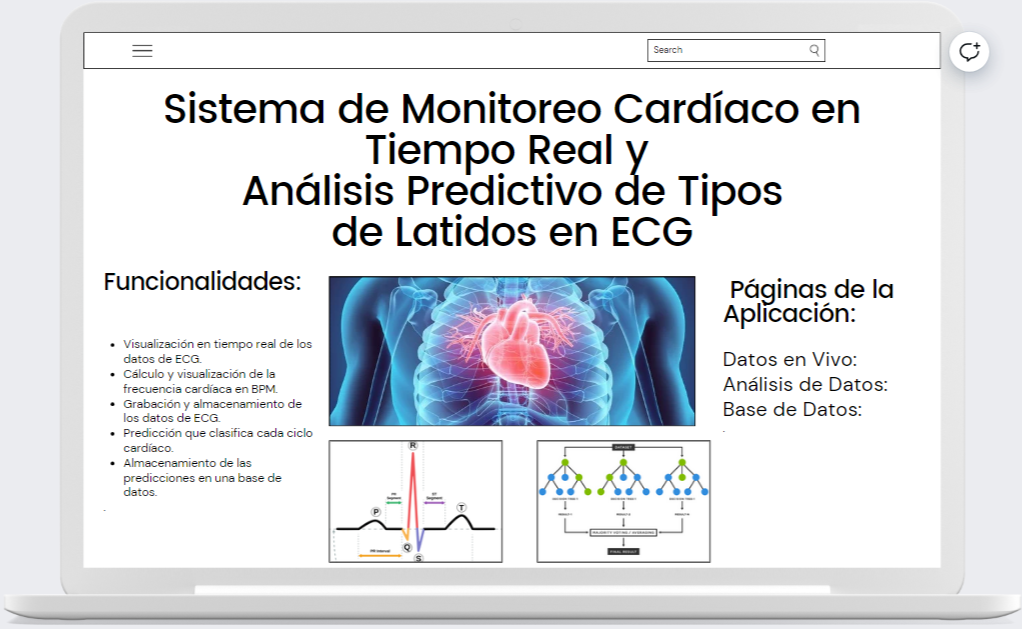
\includegraphics[width=0.8\textwidth]{img/prototipo_interfaz/1.png}
\caption{Pantalla de introducción con opciones de navegación y funcionalidad resumida.}
\label{fig:inicio}
\end{figure}

\begin{figure}[h]
\centering
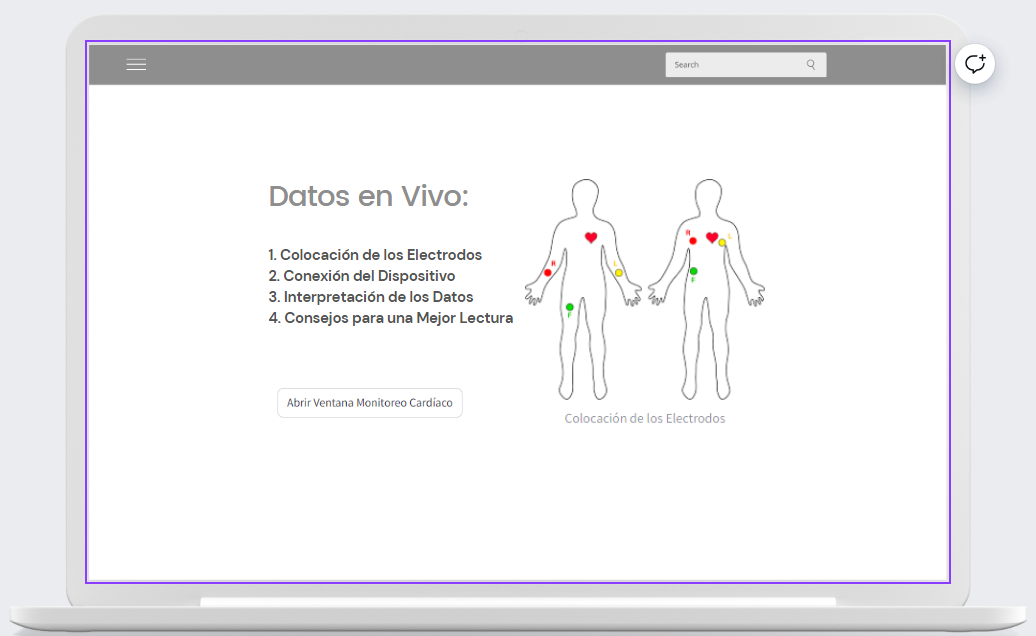
\includegraphics[width=0.8\textwidth]{img/prototipo_interfaz/2.png}
\caption{Interfaz de datos en vivo mostrando la ventana de escritorio Tkinter para visualización de ECG en tiempo real.}
\label{fig:datos-vivo}
\end{figure}

\begin{figure}[h]
\centering
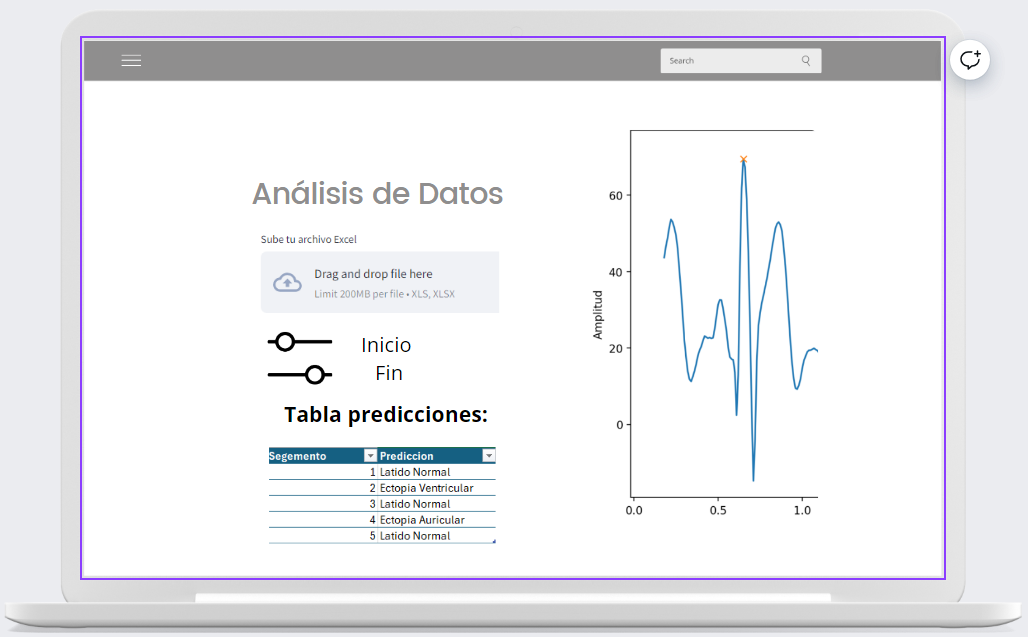
\includegraphics[width=0.8\textwidth]{img/prototipo_interfaz/3.png}
\caption{Pantalla de análisis de datos donde se suben y procesan archivos de ECG para predicciones.}
\label{fig:analisis-datos}
\end{figure}

\begin{figure}[h]
\centering
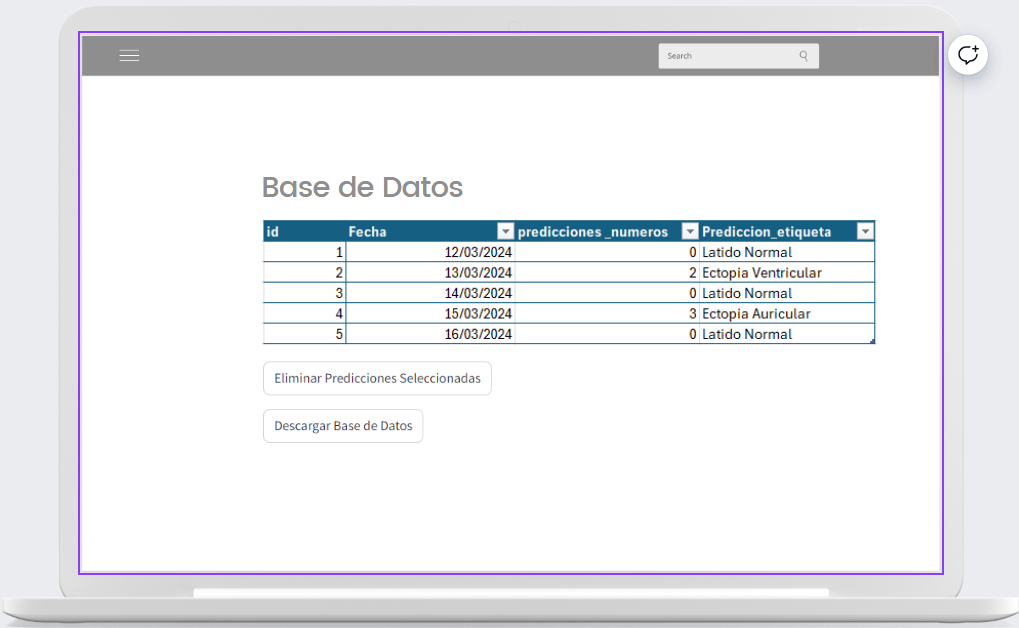
\includegraphics[width=0.8\textwidth]{img/prototipo_interfaz/4.png}
\caption{Interfaz de base de datos para la gestión y visualización de registros almacenados.}
\label{fig:gestion-datos}
\end{figure}

\begin{figure}[h]
\centering
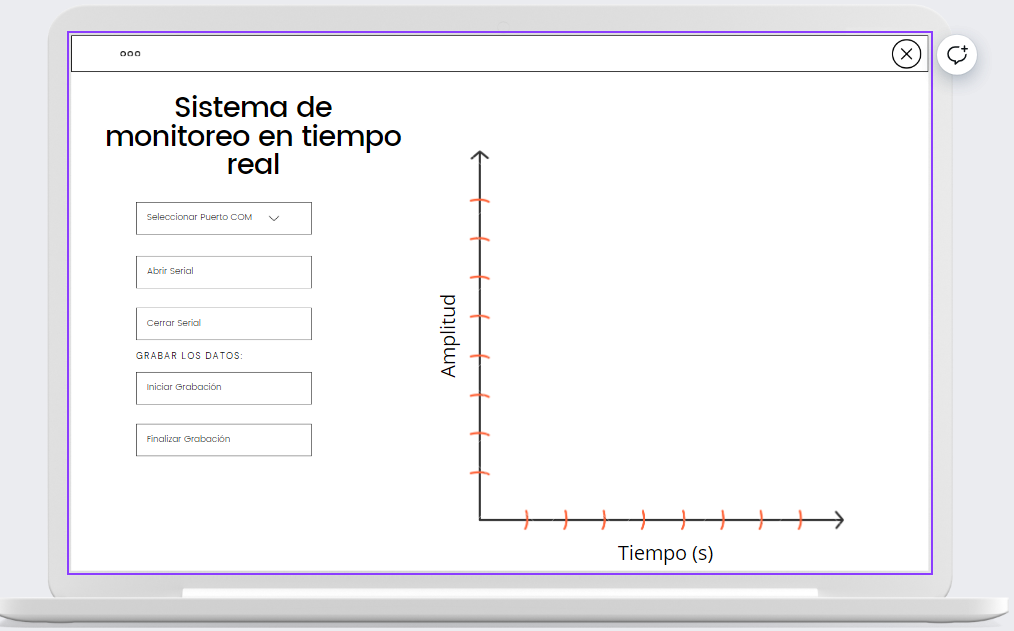
\includegraphics[width=0.8\textwidth]{img/prototipo_interfaz/5.png}
\caption{Configuración y ajustes del sistema para personalización y gestión de cuenta de usuario.}
\label{fig:configuracion}
\end{figure}
